% ============================================================
% 数电实验报告 — 实验六：基于 FPGA 的信号发生器
% ============================================================

\documentclass[12pt]{ctexart}

% --- 宏包 ---
\usepackage{graphicx}
\usepackage{amsmath}
\usepackage{xcolor}
\usepackage{float}
\usepackage{booktabs}
\usepackage{siunitx}
\usepackage{fancyhdr}
\usepackage{caption}
\usepackage{subcaption}
\usepackage{hyperref}
\usepackage{makecell}
\usepackage{enumitem}
\usepackage[outputdir=build]{minted}

\sisetup{per-mode=symbol}

\graphicspath{{./figures/}{../figures/}}

\usepackage[left=2.5cm, right=2.5cm, top=2.5cm, bottom=2.5cm]{geometry}

\setlength{\jot}{6pt}
\setlength{\headheight}{15pt}
\linespread{1.5}
\setlist{nosep}

% --- VHDL 代码样式 ---
\setminted[vhdl]{
    fontsize=\small,
    frame=single,
    linenos,
    breaklines,
    tabsize=4,
    numbersep=8pt,
    xleftmargin=2em
}

% --- 页眉页脚 ---
\pagestyle{fancy}
\fancyhead[C]{数字电子技术实验}
\fancyfoot[C]{\thepage}

\begin{document}

% ==================== 封面 ====================
\thispagestyle{empty}

\begin{figure}[t]
    \centering
    
\includegraphics[width=13cm]{logo1.png}
\end{figure}

\vspace*{\fill}
    \begin{center}
        \Huge\textbf{数字电子技术基础}

        \vspace{0.3cm}
        \Huge\textbf{实验报告}

        \vspace{1cm}
        \LARGE\textbf{实验六：基于 FPGA 的信号发生器}
    \end{center}
\vspace*{\fill}

\begin{table}[H]
    \centering
    \large
    \begin{tabular}{ll}
    \toprule
    \textbf{课程:} & 数字电子技术实验 \\
    \textbf{组员1:} & 郭浩然 2024303980 \\
    \textbf{组员2:} & 庞铭洋 2024302539 \\
    \textbf{组号:} & 15 \\
    \textbf{时间:} & \today \\
    \bottomrule
    \end{tabular}
\end{table}

\newpage

% ==================== 正文 ====================

\section{实验目的}

\begin{enumerate}
    \item 掌握直接数字频率合成 DDS 的查表式波形发生原理，理解用计数器扫描 ROM 地址、把预存采样按顺序读出来重建波形的方法。
    \item 学会用 Quartus II 的 PLL IP 核对板载时钟倍频，掌握用 \texttt{altsyncram} ROM IP 核和 \texttt{.mif} 文件存储波形数据的流程。
    \item 学会用 VHDL 编写地址计数器和数据选择器，再用原理图把 PLL、计数器、ROM、数据选择器连成完整系统，完成文本设计与原理图设计的混合开发。
    \item 理解 8 位 DA 模块 AD9708 把数字码转换为模拟电压的原理，能用拨码开关切换输出波形并用示波器观测验证。
\end{enumerate}

\section{实验要求}

本次实验的要求以现场给出的实验内容为准，具体如下：

\begin{enumerate}
    \item \textbf{要求 1}：配置一块宽度为 8 位的 ROM，在 ROM 中存储 256 个地址的正弦波数据。用 PLL 生成 100\,MHz 时钟作为计数器的计数脉冲，计数器的输出作为地址去读取 ROM 的内容，再把正弦波信号通过 DA 模块 AD9708 转换成模拟信号，通过示波器显示波形。
    \item \textbf{要求 2}：利用控制开关控制波形切换。例如拨动开关置为 0 时输出正弦波，置为 1 时输出其他波形。提示可以用 VHDL 语言写一个数据选择器。
\end{enumerate}

本组在满足要求的基础上做了扩展：一共预存正弦波、三角波、方波和斜坡波四种波形，用 A 和 C 两个拨码开关组成 2 位选择信号，通过 VHDL 写的数据选择器在四种波形之间切换。当 A 与 C 都置 0 时输出正弦波，其余三种组合分别输出另外三种波形。

\section{实验设备}

\begin{itemize}
    \item Quartus II 开发软件，含 MegaWizard Plug-In Manager、PLL IP 核和 ROM IP 核
    \item DE0 开发板，FPGA 型号为 Cyclone V \texttt{5CEBA4F23C7}
    \item USB-Blaster 下载线及计算机
    \item AD9708 高速 8 位 DA 转换子板
    \item RIGOL DHO1204 数字示波器
    \item 板载 50\,MHz 晶振、两个波形选择拨码开关 A 与 C
\end{itemize}

\section{实验原理}

\subsection{DDS 查表式波形发生原理}

直接数字频率合成 DDS 的核心思想是查表：先把一个完整周期的波形按等间隔采样，量化成数字码预存进 ROM；工作时用一个地址计数器在高速时钟驱动下从 0 扫到最大地址再归零，ROM 就按存储顺序循环送出各个采样点，存进去的波形在输出端被逐点重建出来。ROM 只完成地址到数据的映射
\[
    \mathrm{data\_out} = \mathrm{ROM}[\mathrm{addr}],
\]
真正让数据随时间自动输出的是不断累加的地址计数器。

本实验的 ROM 用 Quartus II 的 \texttt{altsyncram} IP 核实现，数据宽度 8 位、存储深度 256 字、地址位宽 8 位，对应 $2^8 = 256$ 个地址。地址计数器 \texttt{Vhdl1} 是一个 8 位模 256 计数器，每来一个时钟上升沿加 1，计满 255 后归零，正好循环扫完 ROM 的 256 个单元，把一个周期的波形重复输出。

\subsection{PLL 倍频与输出波形频率}

DE0 开发板的板载系统时钟为 50\,MHz，要求用 100\,MHz 作为计数脉冲，因此用 PLL IP 核把参考时钟倍频一倍。PLL 以板载 50\,MHz 为参考时钟 \texttt{refclk}，输出 \texttt{outclk\_0} 为 100\,MHz，作为所有计数器和 ROM 的公共时钟。

计数器每 256 个时钟扫完一个周期的波形，所以输出波形的频率为
\[
    f_{\text{out}} = \frac{f_{\text{clk}}}{256} = \frac{100\,\text{MHz}}{256} \approx 390.6\,\text{kHz}.
\]
这就是示波器上观测到的波形重复频率。

\subsection{四种波形的 ROM 数据}

四块 ROM 分别用四个 \texttt{.mif} 文件初始化，每个文件存一个周期对应波形的 256 点 8 位采样，数值范围 $0\sim255$。各波形在几个关键地址上的采样值见表~\ref{tab:wavedata}，由此可以看出它们的形状。

\begin{table}[H]
    \centering
    \caption{四块 ROM 初始化文件与对应波形的特征采样值}
    \label{tab:wavedata}
    \small
    \begin{tabular}{lccccl}
        \toprule
        \textbf{初始化文件} & \textbf{地址 0} & \textbf{地址 64} & \textbf{地址 128} & \textbf{地址 192} & \textbf{波形} \\
        \midrule
        \texttt{dds\_256x8b\_wave.mif}  & 127 & 254 & 127 & 0   & 正弦波 \\
        \texttt{dds\_256x8b\_wave1.mif} & 0   & 128 & 255 & 128 & 三角波 \\
        \texttt{dds\_256x8b\_wave3.mif} & 255 & 255 & 0   & 0   & 方波 \\
        \texttt{dds\_256x8b\_wave4.mif} & 0   & 64  & 128 & 192 & 斜坡波 \\
        \bottomrule
    \end{tabular}
\end{table}

正弦波从中点 127 起，在地址 64 升到峰值 254，地址 128 回到中点，地址 192 降到谷底 0，呈完整正弦变化；三角波从 0 线性升到地址 128 的峰值 255 再线性降回；方波在前半周期保持 255、后半周期保持 0；斜坡波随地址线性递增，从 0 一直到 255。

\subsection{数据选择器与波形切换}

要让一套硬件输出多种波形，关键是在四块 ROM 的输出之间做选择。本实验用 VHDL 写了一个数据选择器 \texttt{bus\_mux}，它有四路 8 位输入总线 \texttt{bus0}$\sim$\texttt{bus3} 和两个选择端 \texttt{sel0}、\texttt{sel1}，根据 \texttt{sel1 sel0} 的组合把其中一路接到 8 位输出 \texttt{dout}。顶层把拨码开关 A 接到 \texttt{sel1}、C 接到 \texttt{sel0}，于是 A 和 C 的四种组合对应四种波形，逻辑见表~\ref{tab:mux}。

\begin{table}[H]
    \centering
    \caption{数据选择器开关组合与输出波形对照}
    \label{tab:mux}
    \begin{tabular}{cccccl}
        \toprule
        \textbf{A (sel1)} & \textbf{C (sel0)} & \textbf{选通总线} & \textbf{数据来源} & \textbf{初始化文件} & \textbf{输出波形} \\
        \midrule
        0 & 0 & \texttt{bus0} & ROM1 & \texttt{dds\_256x8b\_wave.mif}  & 正弦波 \\
        0 & 1 & \texttt{bus1} & ROM2 & \texttt{dds\_256x8b\_wave1.mif} & 三角波 \\
        1 & 0 & \texttt{bus2} & ROM3 & \texttt{dds\_256x8b\_wave3.mif} & 方波 \\
        1 & 1 & \texttt{bus3} & ROM4 & \texttt{dds\_256x8b\_wave4.mif} & 斜坡波 \\
        \bottomrule
    \end{tabular}
\end{table}

四块 ROM 各配一个地址计数器，全部接同一路 100\,MHz 时钟并同步计数，所以它们时刻输出相同地址、各自读出本通路的波形采样，数据选择器只是把被选中的那一路送到输出，切换开关即可在不停机的情况下实时换波形。

\subsection{DA 转换原理}

ROM 输出的是 8 位数字码，要在示波器上看到模拟波形还需要数模转换。AD9708 是一片高速 8 位 DA 转换器，它把输入的 8 位二进制码按比例转换成模拟电流并经外围电路变成电压，输出电压与数字码近似成正比
\[
    V_{\text{out}} \approx \frac{D}{2^{8}} \, V_{\text{ref}},
\]
其中 $D$ 为输入的数字码、$V_{\text{ref}}$ 为满量程参考。计数器每个时钟更新一个 ROM 采样，AD9708 就对应输出一个电压台阶，256 个台阶连起来就重建出一个周期的模拟波形，台阶经示波器带宽平滑后即为光滑的波形曲线。

\section{实验内容}

本系统把 VHDL 文本设计和原理图设计结合起来：地址计数器和数据选择器用 VHDL 编写，PLL 和 ROM 用 IP 核生成，编译后各自生成原理图符号，再在顶层原理图中调用并连线，拼成完整系统。整个软件流程是建立工程，配置 PLL 和四块 ROM IP 核，编写各模块 VHDL 代码并生成符号，绘制顶层原理图，编译，引脚分配，下载到开发板，最后接 DA 模块和示波器观测。

\subsection{建立工程与配置 IP 核}

打开 Quartus II，用 \textbf{File $\rightarrow$ New Project Wizard} 新建工程，器件选 DE0 开发板对应的 Cyclone V \texttt{5CEBA4F23C7}。随后配置两类 IP 核：

\begin{enumerate}
    \item \textbf{PLL IP 核}：用 MegaWizard 生成一个锁相环，参考时钟频率设为 50\,MHz，输出 \texttt{outclk\_0} 设为 100\,MHz，把板载时钟倍频一倍后作为全局计数脉冲。
    \item \textbf{四块 ROM IP 核}：按 \texttt{ROM: 1-PORT} 类型各配一块，输出位宽都设为 8 位、深度都设为 256 字、地址 8 位，并分别勾选用 \texttt{.mif} 文件初始化，依次指定 \texttt{dds\_256x8b\_wave.mif}、\texttt{dds\_256x8b\_wave1.mif}、\texttt{dds\_256x8b\_wave3.mif}、\texttt{dds\_256x8b\_wave4.mif}。这四个 \texttt{.mif} 里的采样值不是手工填的，而是用波形转 MIF 上位机软件从一个周期的目标波形生成，幅值范围 $0\sim255$。正弦波 \texttt{.mif} 的前几个采样值列在表~\ref{tab:sinmif}。
\end{enumerate}

\begin{table}[H]
    \centering
    \caption{正弦波 ROM 初始化文件 \texttt{dds\_256x8b\_wave.mif} 部分采样值}
    \label{tab:sinmif}
    \begin{tabular}{ccccccccc}
        \toprule
        地址 & 0 & 1 & 2 & 3 & 4 & 5 & 6 & 7 \\
        \midrule
        十进制数据 & 127 & 130 & 133 & 136 & 139 & 142 & 145 & 148 \\
        \bottomrule
    \end{tabular}
\end{table}

\subsection{编写 VHDL 子模块}

\subsubsection{8 位地址计数器 Vhdl1}

\texttt{Vhdl1} 负责产生 ROM 的 8 位地址。计数脉冲每来一个上升沿就加 1，数到 255 后归零并给出一个进位脉冲 \texttt{COUT}，这样循环扫完 256 个地址；复位端 \texttt{RST} 低电平有效，顶层把它接到 VCC，让计数器始终不复位、保持正常计数。

\begin{minted}{vhdl}
LIBRARY IEEE;
USE IEEE.STD_LOGIC_1164.ALL;
USE IEEE.STD_LOGIC_UNSIGNED.ALL;
ENTITY Vhdl1 IS
    PORT ( clk,RST : IN  STD_LOGIC;
           DOUT    : OUT STD_LOGIC_VECTOR (7 DOWNTO 0);  -- 8位计数
           COUT    : OUT STD_LOGIC);                      -- 进位位
END Vhdl1;
ARCHITECTURE fwm OF Vhdl1 IS
    SIGNAL Q1 : STD_LOGIC_VECTOR (7 DOWNTO 0);
BEGIN
    PROCESS(clk,RST)
    BEGIN
        IF RST = '0' THEN
            Q1 <= (OTHERS => '0'); COUT <= '0';
        ELSIF clk'EVENT AND clk = '1' THEN
            Q1 <= Q1 + 1;
            COUT <= '0';
            IF Q1 >= "11111111" THEN          -- 计满 255 归零
                Q1 <= (OTHERS => '0'); COUT <= '1';
            END IF;
        END IF;
    END PROCESS;
    DOUT <= Q1;
END fwm;
\end{minted}
\captionof{listing}{8 位地址计数器 Vhdl1.vhd}
\label{lst:vhdl1}

\subsubsection{四选一数据选择器 bus\_mux}

\texttt{bus\_mux} 接收四块 ROM 的 8 位输出 \texttt{bus0}$\sim$\texttt{bus3} 和两个选择端 \texttt{sel0}、\texttt{sel1}，用一段组合逻辑根据 \texttt{sel1 sel0} 把对应通路接到输出 \texttt{dout}，实现表~\ref{tab:mux} 的波形选择。

\begin{minted}{vhdl}
LIBRARY IEEE;
USE IEEE.STD_LOGIC_1164.ALL;
ENTITY bus_mux IS
PORT (
    bus0  : IN  STD_LOGIC_VECTOR(7 DOWNTO 0);   -- 4 路 8 位输入总线
    bus1  : IN  STD_LOGIC_VECTOR(7 DOWNTO 0);
    bus2  : IN  STD_LOGIC_VECTOR(7 DOWNTO 0);
    bus3  : IN  STD_LOGIC_VECTOR(7 DOWNTO 0);
    sel0  : IN  STD_LOGIC;                       -- 两个独立的选择输入
    sel1  : IN  STD_LOGIC;
    dout  : OUT STD_LOGIC_VECTOR(7 DOWNTO 0)     -- 8 位输出总线
);
END bus_mux;
ARCHITECTURE Behavioral OF bus_mux IS
BEGIN
    PROCESS(bus0, bus1, bus2, bus3, sel0, sel1)
    BEGIN
        IF    sel1 = '0' AND sel0 = '0' THEN dout <= bus0;
        ELSIF sel1 = '0' AND sel0 = '1' THEN dout <= bus1;
        ELSIF sel1 = '1' AND sel0 = '0' THEN dout <= bus2;
        ELSIF sel1 = '1' AND sel0 = '1' THEN dout <= bus3;
        ELSE  dout <= (OTHERS => '0');
        END IF;
    END PROCESS;
END Behavioral;
\end{minted}
\captionof{listing}{四选一数据选择器 bus\_mux.vhd}
\label{lst:busmux}

把这两个模块和 PLL、四块 ROM 分别编译，再用 \textbf{File $\rightarrow$ Create/Update $\rightarrow$ Create Symbol Files for Current File} 各自生成 \texttt{.bsf} 符号，供顶层原理图调用。

\subsection{绘制顶层原理图}

新建一个 BDF 原理图作为顶层设计，把各模块符号放上去并按下面的关系连线，顶层原理图如图~\ref{fig:top}。

\begin{itemize}
    \item 输入有三个：\texttt{clk} 接板载 50\,MHz 系统时钟，A 和 C 接两个波形选择拨码开关。
    \item PLL 以 \texttt{clk} 为参考时钟，输出 100\,MHz，并经一个 \texttt{Clk\_100MHz} 输出端引出作测试点；这路 100\,MHz 时钟同时扇出到四个计数器和四块 ROM，作为公共计数脉冲和读时钟。
    \item 四个 \texttt{Vhdl1} 计数器的 \texttt{DOUT[7..0]} 分别接 ROM1$\sim$ROM4 的 \texttt{address[7..0]}，四个计数器的 \texttt{RST} 都接 VCC，始终计数。
    \item ROM1$\sim$ROM4 的输出 \texttt{q[7..0]} 分别接 \texttt{bus\_mux} 的 \texttt{bus0}$\sim$\texttt{bus3}；A 接 \texttt{sel1}，C 接 \texttt{sel0}。
    \item \texttt{bus\_mux} 的 \texttt{dout[7..0]} 接 8 位输出总线 \texttt{a[7..0]}，再拆成输出脚 0$\sim$7 送 AD9708 的数据口 D0$\sim$D7。
\end{itemize}

\begin{figure}[H]
    \centering
    
\includegraphics[width=0.98\textwidth]{电路图.png}
    \caption{基于 FPGA 的信号发生器顶层原理图}
    \label{fig:top}
\end{figure}

\subsection{编译、引脚分配与下载}

把 BDF 设为顶层实体完整编译一遍，再打开 Pin Planner 按表~\ref{tab:pins} 把各端口锁定到 DE0 开发板和 DA 子板对应的引脚上。其中输出脚 0$\sim$7 是 8 位数据的低位到高位，依次接 AD9708 的 D0$\sim$D7。

\begin{table}[H]
    \centering
    \caption{引脚分配：端口与 DE0 板载资源及 DA 模块的对应关系}
    \label{tab:pins}
    \begin{tabular}{llll}
        \toprule
        \textbf{端口} & \textbf{方向} & \textbf{引脚} & \textbf{说明} \\
        \midrule
        \texttt{clk}         & 输入 & \texttt{PIN\_M9}   & 板载 50\,MHz 系统时钟，PLL 参考时钟 \\
        A                    & 输入 & \texttt{PIN\_AB13} & 波形选择开关，接 \texttt{sel1} \\
        C                    & 输入 & \texttt{PIN\_AB12} & 波形选择开关，接 \texttt{sel0} \\
        \texttt{Clk\_100MHz} & 输出 & \texttt{PIN\_M22}  & PLL 100\,MHz 时钟测试点 \\
        0                    & 输出 & \texttt{PIN\_K17}  & DA 数据 D0 \\
        1                    & 输出 & \texttt{PIN\_L17}  & DA 数据 D1 \\
        2                    & 输出 & \texttt{PIN\_M18}  & DA 数据 D2 \\
        3                    & 输出 & \texttt{PIN\_P17}  & DA 数据 D3 \\
        4                    & 输出 & \texttt{PIN\_P19}  & DA 数据 D4 \\
        5                    & 输出 & \texttt{PIN\_N19}  & DA 数据 D5 \\
        6                    & 输出 & \texttt{PIN\_T22}  & DA 数据 D6 \\
        7                    & 输出 & \texttt{PIN\_R22}  & DA 数据 D7 \\
        \bottomrule
    \end{tabular}
\end{table}

重新编译后接上 USB-Blaster，用 JTAG 模式把 \texttt{.sof} 配置文件下载到 DE0 开发板。

\subsection{接 DA 模块与示波器观测}

把 AD9708 子板的数据口接到输出脚 0$\sim$7，子板的模拟输出经 SMA 接到 RIGOL DHO1204 示波器。逐一拨动 A 和 C 两个开关，示波器上分别观测到四种波形，结果如图~\ref{fig:waves}。

\begin{figure}[H]
    \centering
    \begin{subfigure}{0.48\textwidth}
        \centering
        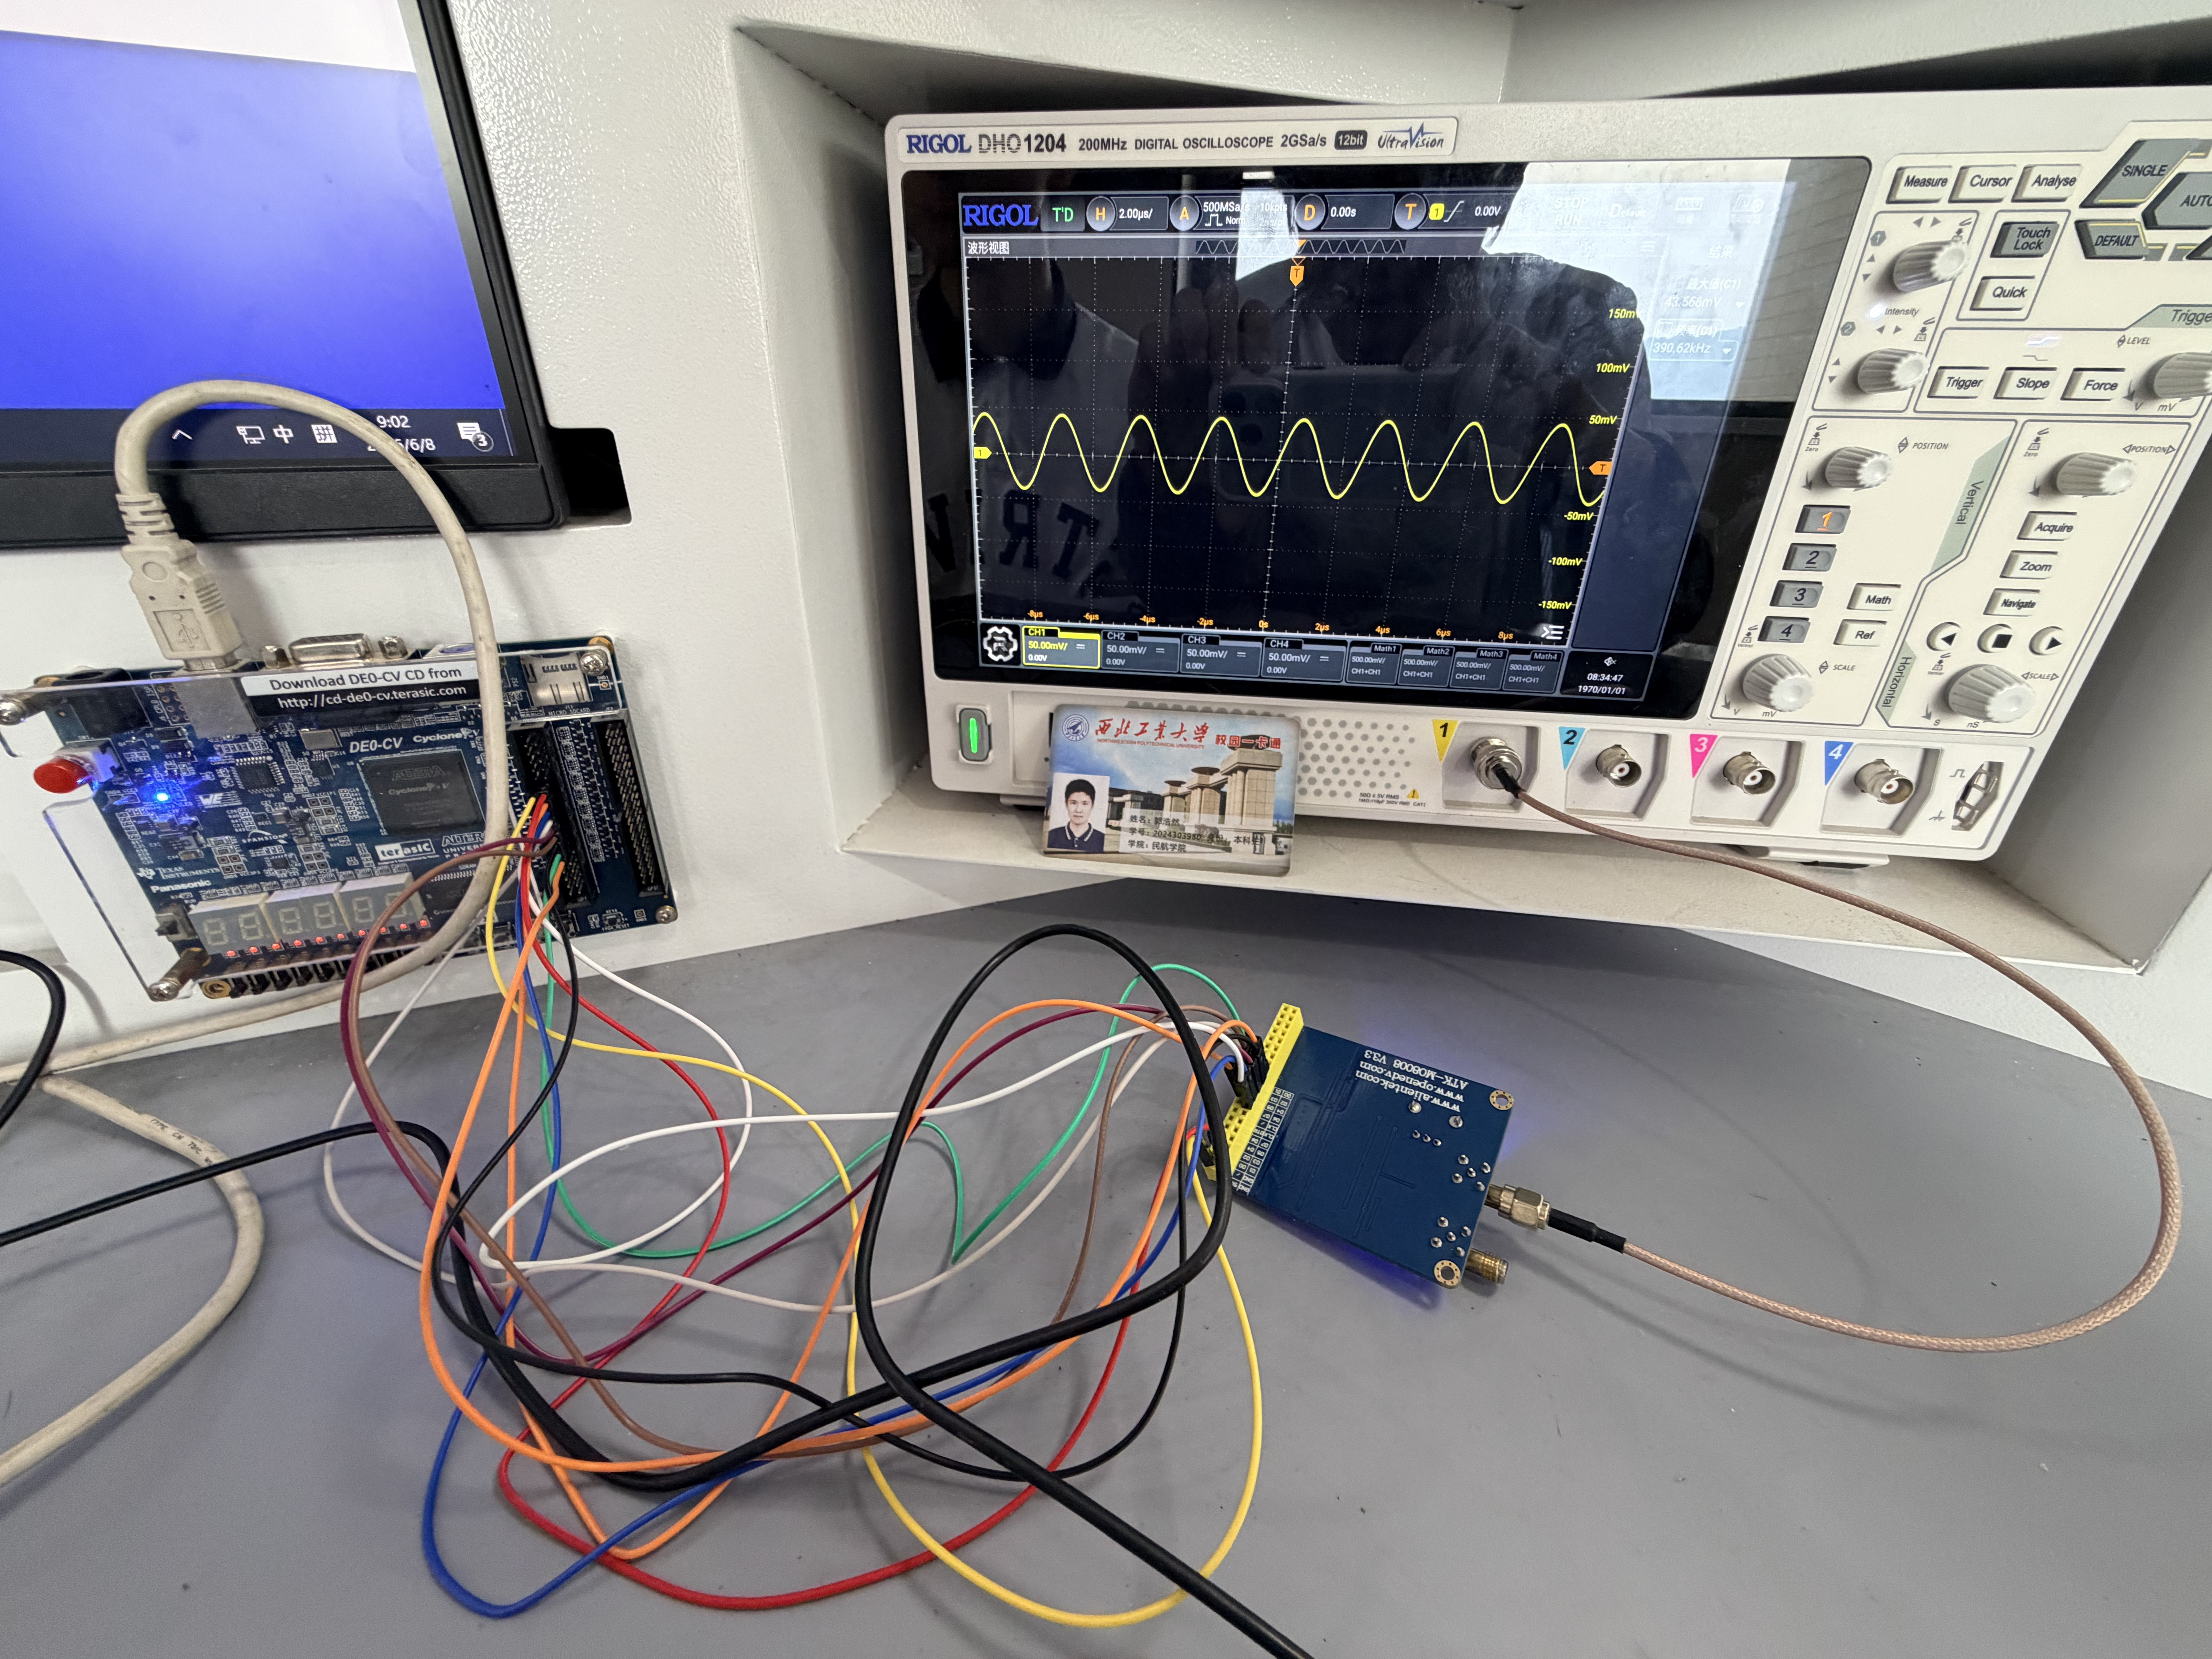
\includegraphics[width=\linewidth]{正弦波.jpg}
        \caption{正弦波输出，A = 0，C = 0}
    \end{subfigure}\hfill
    \begin{subfigure}{0.48\textwidth}
        \centering
        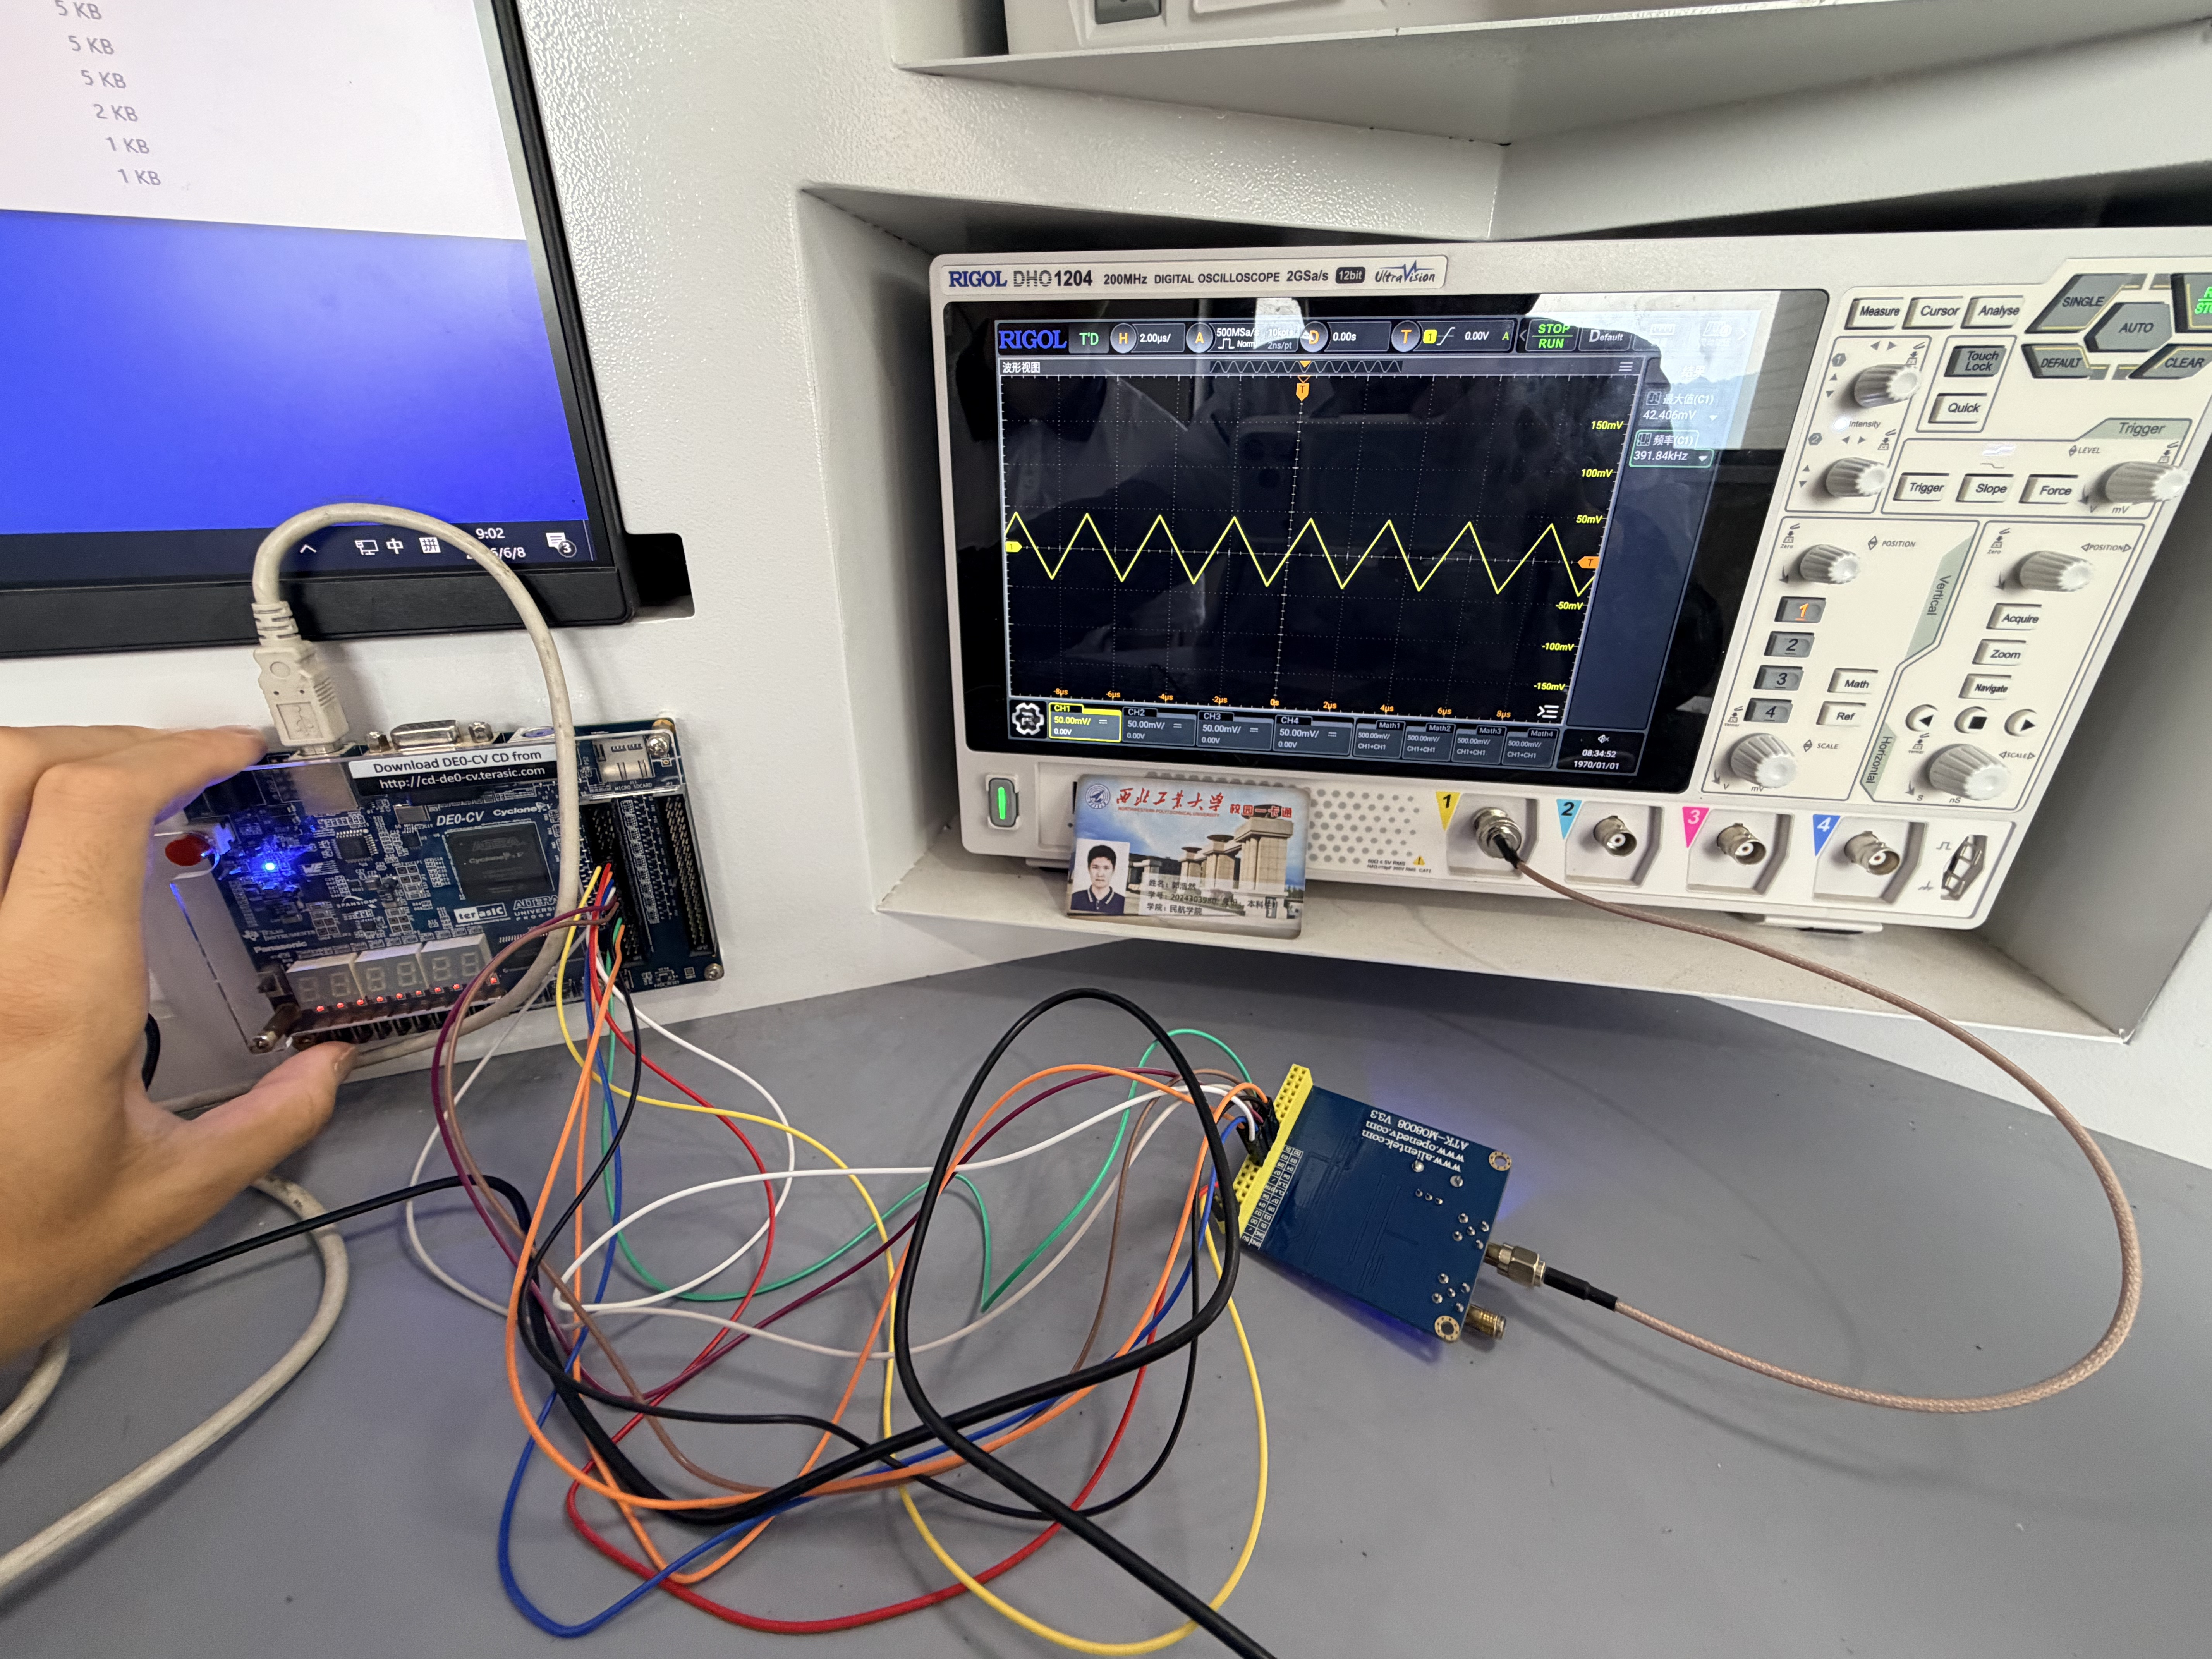
\includegraphics[width=\linewidth]{三角波.jpg}
        \caption{三角波输出，A = 0，C = 1}
    \end{subfigure}

    \vspace{6pt}
    \begin{subfigure}{0.48\textwidth}
        \centering
        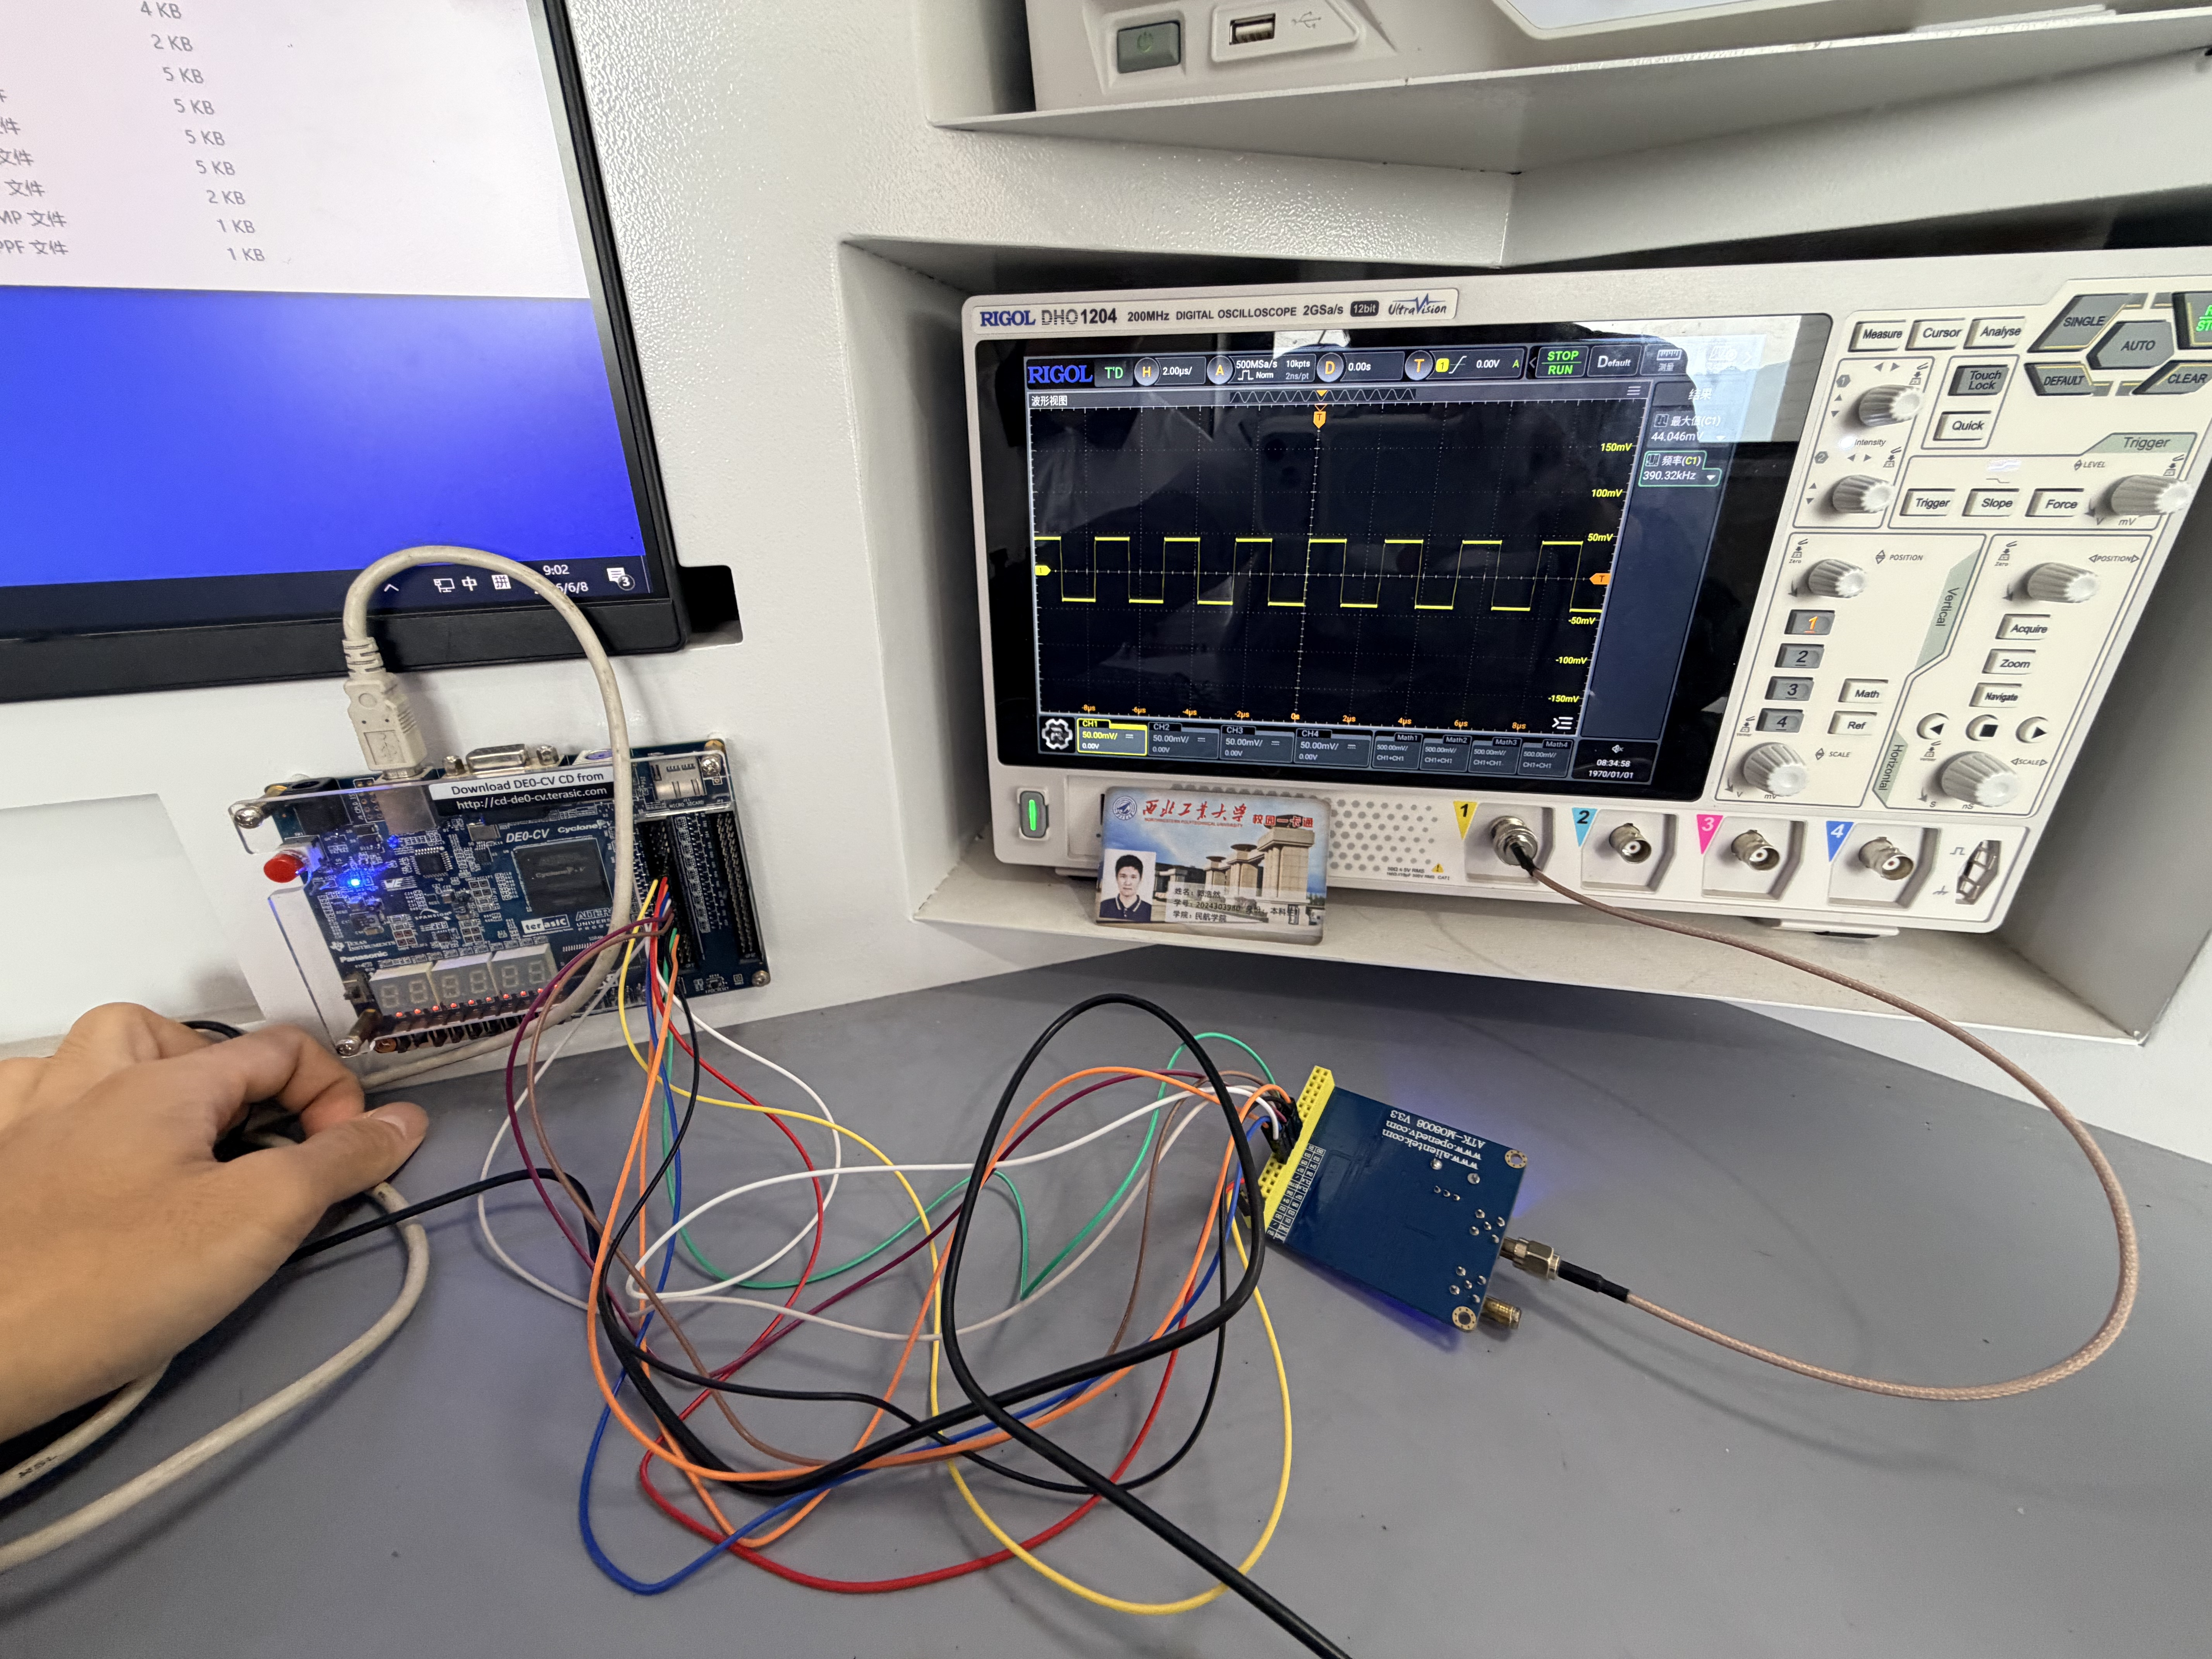
\includegraphics[width=\linewidth]{方波.jpg}
        \caption{方波输出，A = 1，C = 0}
    \end{subfigure}\hfill
    \begin{subfigure}{0.48\textwidth}
        \centering
        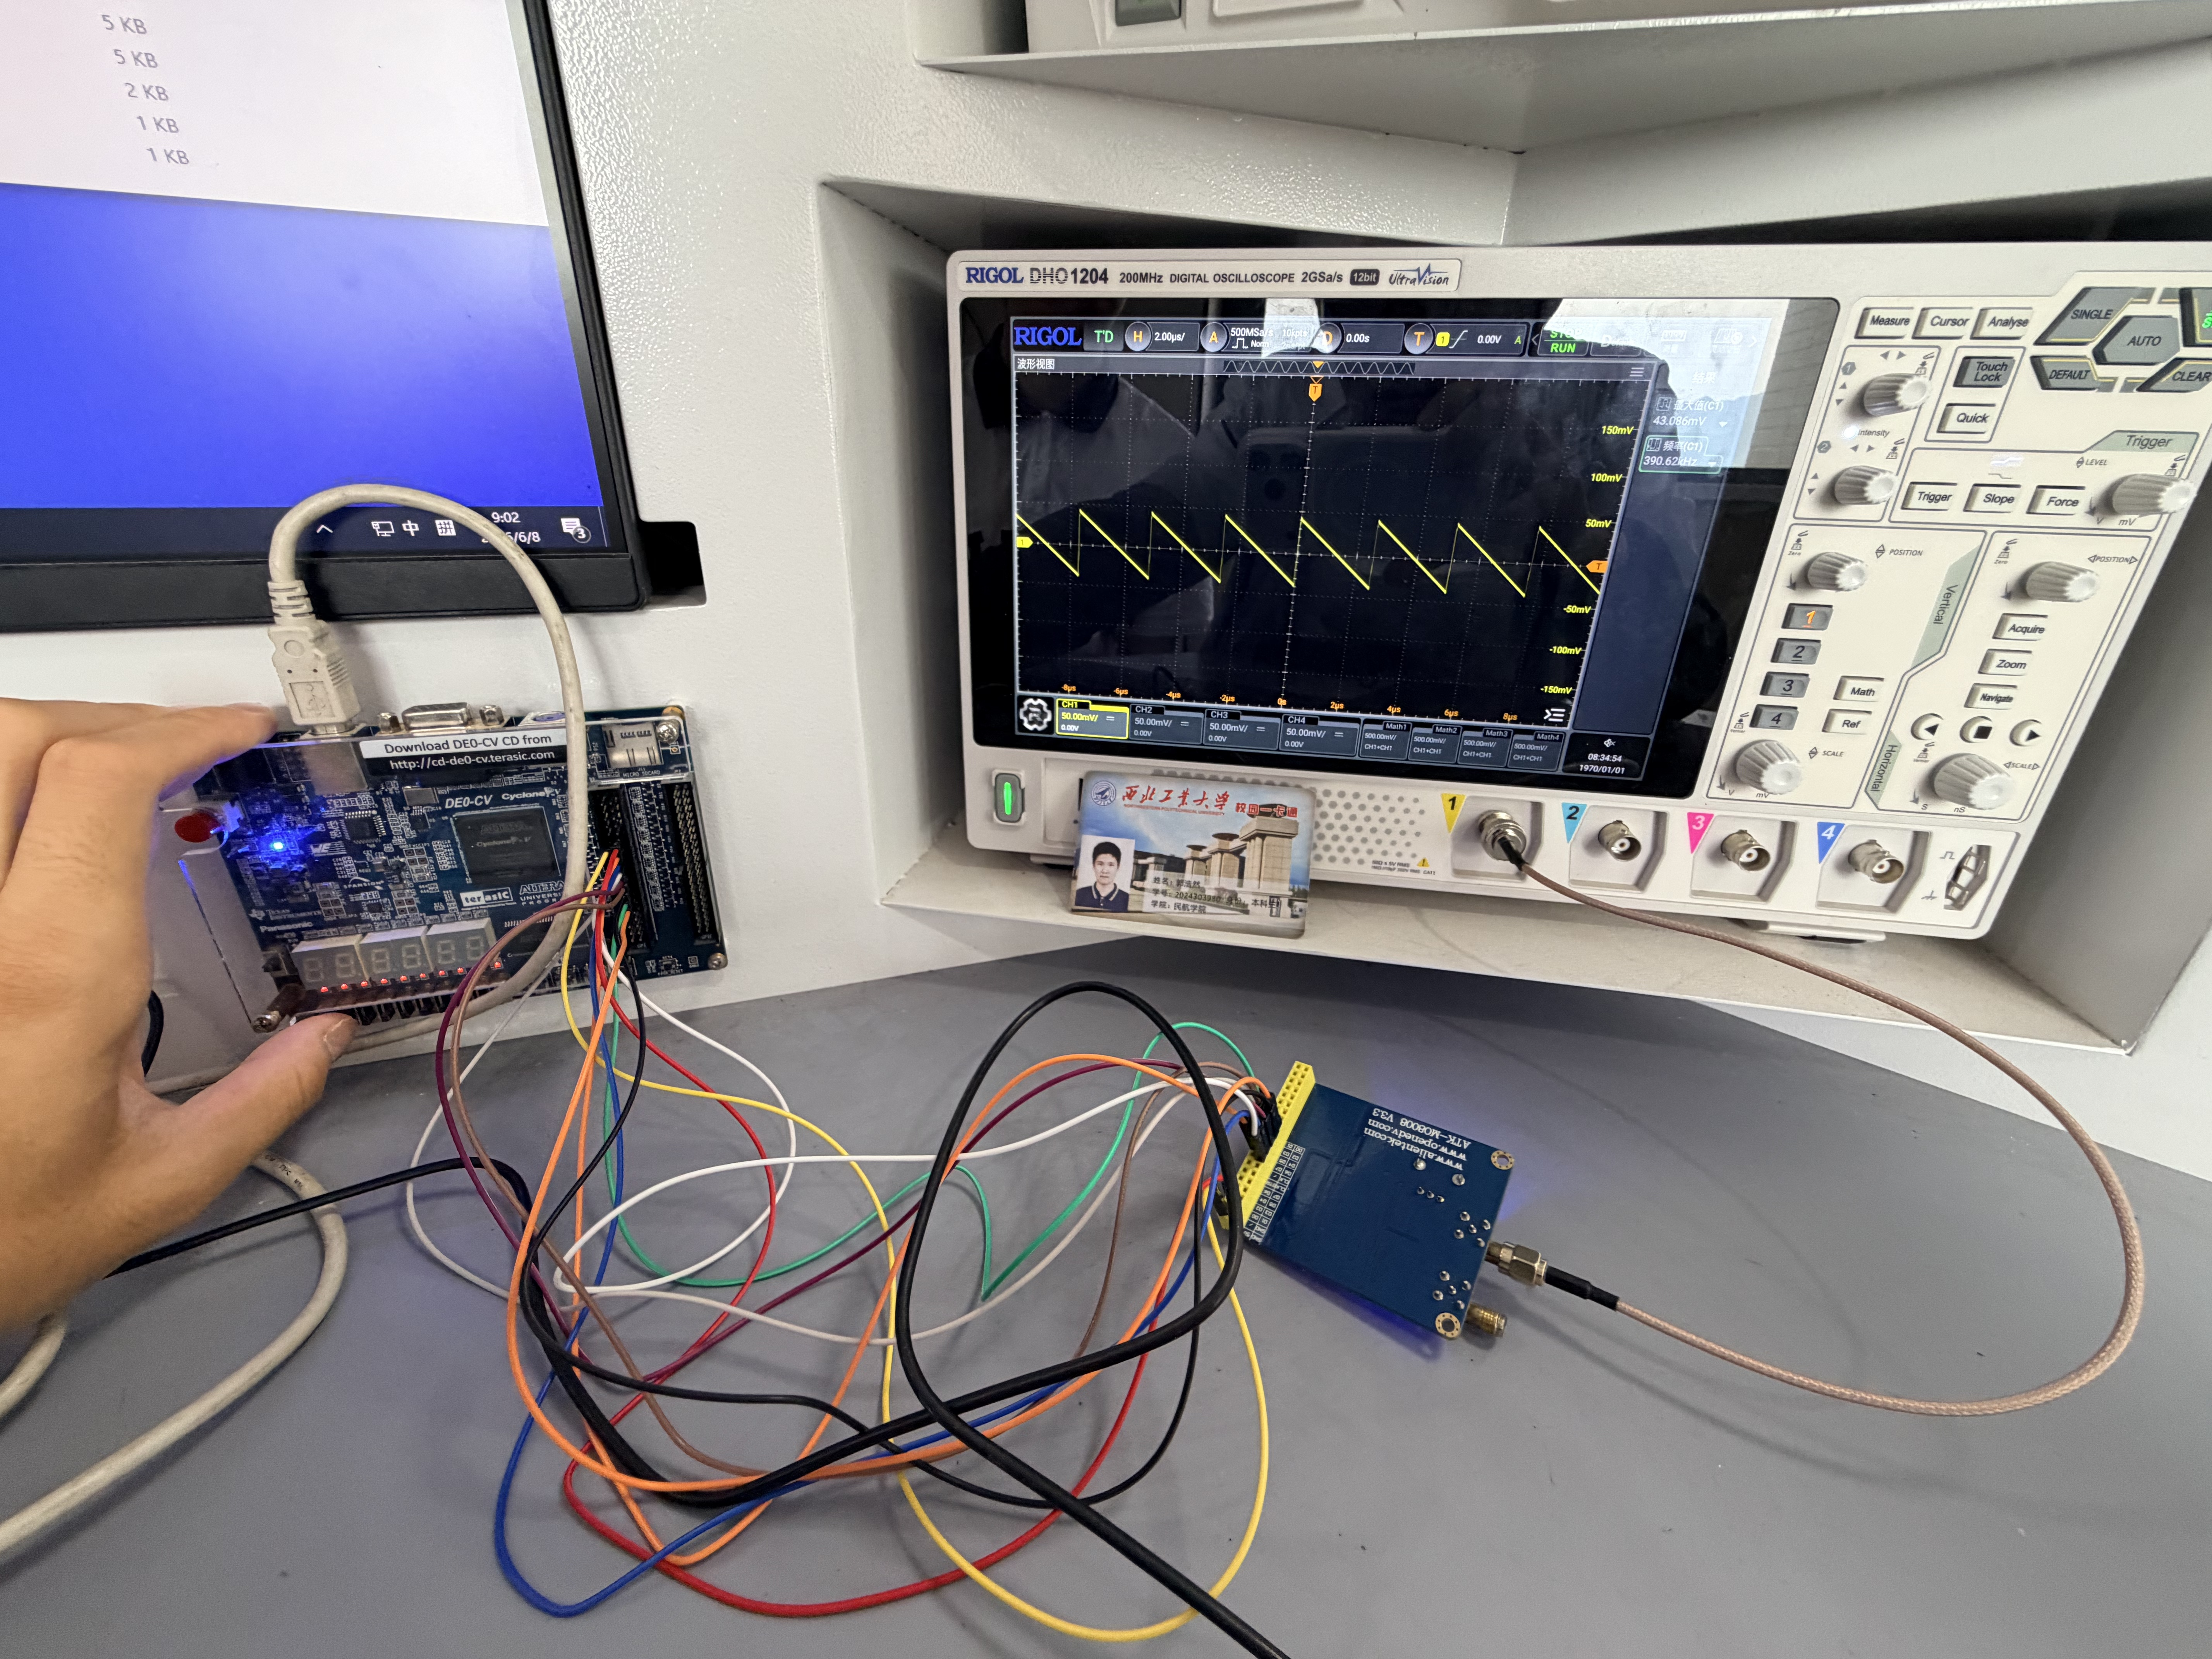
\includegraphics[width=\linewidth]{斜坡信号.jpg}
        \caption{斜坡波输出，A = 1，C = 1}
    \end{subfigure}
    \caption{四种波形的示波器实测结果}
    \label{fig:waves}
\end{figure}

\subsection{数据分析}

把示波器实测波形与表~\ref{tab:wavedata} 中各 ROM 预存的采样数据逐一对照，可以看出实测结果与设计完全吻合：

\begin{itemize}
    \item A 与 C 都为 0 时选通 ROM1，示波器显示一条光滑的正弦波，与 \texttt{dds\_256x8b\_wave.mif} 中从中点升到峰值再降到谷底的采样规律一致。
    \item A 为 0、C 为 1 时选通 ROM2，显示对称的三角波，对应 \texttt{dds\_256x8b\_wave1.mif} 中先线性上升到 255 再线性下降的数据。
    \item A 为 1、C 为 0 时选通 ROM3，显示方波，对应 \texttt{dds\_256x8b\_wave3.mif} 中前半周期为 255、后半周期为 0 的数据。
    \item A 为 1、C 为 1 时选通 ROM4，显示斜坡波，每个周期电压随地址线性升到满量程后迅速跌回，对应 \texttt{dds\_256x8b\_wave4.mif} 的线性递增数据。
\end{itemize}

四种波形拨动开关即可实时切换，互不干扰，验证了数据选择器和多 ROM 查表结构的正确性。波形频率约为 100\,MHz 除以 256，即 390.6\,kHz 量级，与理论计算相符。由于 DA 输出本质是 256 级电压台阶，在示波器上仔细看仍可见细小的阶梯，幅度越平缓的波形阶梯越明显，这是 8 位量化和有限采样点共同造成的，提高位宽或采样点数可以让波形更光滑。

\section{实验过程中的问题}

\begin{enumerate}
    \item \textbf{用 PLL 产生 100\,MHz 计数脉冲}。板载晶振只有 50\,MHz，要按要求得到 100\,MHz 必须借助 PLL 倍频。配置时把参考时钟设为 50\,MHz、输出设为 100\,MHz，综合后用 \texttt{Clk\_100MHz} 引出测试点确认时钟正常，再把它作为计数器和 ROM 的公共时钟。
    \item \textbf{\texttt{.mif} 文件要与 ROM 参数对上}。\texttt{.mif} 里的 \texttt{WIDTH} 和 \texttt{DEPTH} 必须与 ROM IP 的位宽 8、深度 256 一致，地址和数据的基数也要写对，否则综合时会报初始化数据无法识别的错误。四个 \texttt{.mif} 都用波形转 MIF 上位机软件从目标波形直接生成，省去手工填 256 个数据，也避免填错。
    \item \textbf{DA 数据线位序的对应}。AD9708 的数据口 D0$\sim$D7 要和输出脚 0$\sim$7 一一对应，如果高低位接反，输出波形会被镜像或失真。接线时按表~\ref{tab:pins} 的对应关系逐根核对，确认低位脚接 D0、高位脚接 D7。
    \item \textbf{开关组合与波形的对应关系}。数据选择器用 A 接 \texttt{sel1}、C 接 \texttt{sel0}，刚开始容易把两个开关的高低位记混，导致切出来的波形和预期不符。对照表~\ref{tab:mux} 把每种组合实测一遍，确认四种波形都能正确切换。
\end{enumerate}

\section{心得体会}

\begin{enumerate}
    \item 这次实验让我把 DDS 查表式波形发生的思路理解得更透彻。把一个周期的波形采样预存进 ROM，再用计数器顺序扫描地址，就能不断重建出任意波形，正弦波、三角波、方波、斜坡波只是换了 \texttt{.mif} 里的数据而已。这种存采样、扫地址的方法是函数信号发生器的基础。
    \item 配置 PLL 和 ROM 这两类 IP 核，让我熟悉了 MegaWizard 的用法。用 PLL 可以方便地把板载时钟倍频到需要的频率，用 ROM IP 核可以直接调用 FPGA 内部的专用存储块来存波形，比自己用逻辑搭建省资源也更可靠。
    \item 整个系统是 VHDL 文本设计与原理图设计的结合：计数器和数据选择器的逻辑用 VHDL 描述更清晰，PLL、ROM、多个模块之间怎么连用原理图看得更直观。再加上 AD9708 把数字码还原成模拟波形，我完整走通了从数字设计到数模转换、再到示波器观测的全链路，对数字系统的整体设计流程熟悉了不少。
\end{enumerate}

\end{document}
